\section{Moorer}

Il testo\footcite{jm:rev} di \jam non è completo e preciso come il
testo\footcite{ms:rev62} di \ms. Tuttavia, è significativo riportare almeno
le implementazioni di efficienza relative al numero dei moltiplicatori impiegati
nella realizzazione degli \emph{All-Pass} che concorrente all'aumento delle
risorse informatiche disponibili al tempo, consente l'introduzione di piccoli
filtri all'interno del sistema di riverberazione.

\subsection{\emph{All-Pass} a un moltiplicatore}

\lstinputlisting{Code/amapf.dsp}

\begin{figure}[htp]
\centering
\includegraphics[width=1\textwidth]{Code/amapf-svg/process.pdf}
\caption{All Pass \emph{one-multiply} descritto da \jam}
\label{fig:amapf}
\end{figure}

\subsection{\emph{All-Pass} oscillante}

\lstinputlisting{Code/amapfo.dsp}

\begin{figure}[htp]
\centering
\includegraphics[width=1\textwidth]{Code/amapfo-svg/process.pdf}
\caption{All Pass \emph{oscillante} descritto da \jam}
\label{fig:amapfo}
\end{figure}

\subsection{\emph{Comb} con filtro}

\lstinputlisting{Code/amcomblp.dsp}

\begin{figure}[htp]
\centering
\includegraphics[width=1\textwidth]{Code/amcomblp-svg/process.pdf}
\caption{\emph{Comb} con filtro}
\label{fig:amcombfir}
\end{figure}
